%++++++++++++++++++++++++++++++++++++++++
% Don't modify this section unless you know what you're doing!
\documentclass[letterpaper,12pt]{article}
\usepackage{tabularx} % extra features for tabular environment
\usepackage{amsmath}  % improve math presentation
\usepackage{graphicx} % takes care of graphic including machinery
\usepackage[margin=1in,letterpaper]{geometry} % decreases margins
\usepackage{cite} % takes care of citations
\usepackage[final]{hyperref} % adds hyper links inside the generated pdf file
\hypersetup{
	colorlinks=true,       % false: boxed links; true: colored links
	linkcolor=blue,        % color of internal links
	citecolor=blue,        % color of links to bibliography
	filecolor=magenta,     % color of file links
	urlcolor=blue         
}
\usepackage{parskip}
%++++++++++++++++++++++++++++++++++++++++


\begin{document}

\title{IE598 Project Report \\ Measure Similarity Among Images}
\author{Zhe Sun}
\date{May 1, 2016}
\maketitle

\begin{abstract}

The main purpose of this study is to explore the feasibility of measuring similarity among images in a large image dataset. First, a basic implementation of measuring image similarity based on the Hamming distance of their hash values was performed in this project. Three different hashing algorithms were evaluated based on their false-positive ratio and effectiveness. The experiment results demonstrated that given a query image, similar images in the image dataset could be successfully extracted using all of the three hashing algorithms. Further studies were conducted to apply the MinHash signature to estimate the Jaccard Similarity between two sets of images.

\end{abstract}


\section{Introduction}

In the past few decades, a huge amount of images have been created on the Internet. Images are ubiquitous, and a lot of efforts have been put into the management of images. One of the most important concepts in image management is to automatically detect whether two images are similar. By successfully implementing the image comparison mechanism, a lot of applications such as image filters and image search engine could be accomplished. During the IE598 class, an approach to find similar items in structured data sets using their MinHash signatures has been discussed. An example of estimating the Jaccard Similarity between two sets of sentences using their MinHash signatures was shown in the course notes. In this project, this approach was extended to measure the similarity between two datasets of images. Finding the set similarity for the image datasets requires a hashing algorithm for the images, thus a discussion of choosing the appropriate hashing methods was also provided in the first part of this report. Three different hashing algorithms were compared by conducting experiments to look for images which are similar to the query image in an image dataset using different hashing methods. The chosen hashing algorithm was then used to generate the MinHash signatures for a set of images. In the next part of this study, the Jaccard Similarity between two sets of images was estimated by comparing the MinHash signatures of these two image datasets, which were generated in the previous step. 
 
\section{Image Hashing}

The purpose of image hashing is to create a unique identifier for an image by evaluating the contents of the image. Given an input image, a hash function will be used to compute an image hash based on the image’s visual appearance and graphical components. The size, color, brightness and structure of the image will determine the value of the image hash. An ideal image hashing function will generate ``similar" hash values for images that are similar in their appearance. Conventional cryptographic hashing algorithms such as Message Digest (MD) and Secure Hash Function (SHA) do not serve the purpose because even a very small change in the input image will result in a significantly different hash value. An example is provided in \href{http://blog.iconfinder.com/detecting-duplicate-images-using-python/}{here} to illustrate that even a minor change in the color of a small component of the graph will result in a completely different hash value.

Therefore, a good hash function is required to conduct the image similarity search. The following \href{http://www.hackerfactor.com/blog/?/archives/529-Kind-of-Like-That.html}{webpage} introduces three commonly adopted image hashing methods: Perceptive Hash, Average Hash and Difference Hash.

\textbf{Average Hash (aHash): } The color and size of the image is reduced and shrunk to a gray-scale 8x8 square and the mean value of the 64 colors is computed as the average color. It then sets 64 bits in the hash value based on whether each pixel's color value is greater or less than the average color for the image. A 64-bit integer hash value is then constructed. The resulting hash value is pretty consistent even if the size or aspect ratio of the image changes. A minor change in the brightness or color will not alter the hash value significantly.

\textbf{Perceptive Hash (pHash): } The discrete cosine transform (DCT) is used to be evaluated based on the frequencies rather than color values of the image. The size and color of the image are reduced first, and its DCT is computed and reduced. A 64-bit hash value is then constructed based on whether the DCT of each pixel is greater than the average value.

\textbf{Difference Hash (dHash): } This hash function is similar to aHash, with the gradient of the image is of interest instead of the color. The image is first reduced in color and shrunk in size, and the difference between adjacent pixels is computed by identifying the relative gradient direction. The hash value is computed based on whether the left pixel is brighter than the right pixel. 

The author of this blog has commented that the runtime of the dHash algorithm is significantly faster than the other two algorithms. The author also conducted experiments to evaluate the accuracy of these three hash algorithms. He concludes that dHash yields the best results with very few false positives. In order to verify his observation, several experiments were conducted to examine the accuracy of these three image hash algorithms, and the experiment results are presented in the next section.


\section{Experiments}

The image dataset used in this study is the legendary \href{http://www.vision.caltech.edu/Image_Datasets/Caltech101/}{CALTECH-101 dataset}. It contains over 7,500 images from 101 different categories including human faces, traffic signs, animals, flowers and vehicles. Among the 7,500 images, I manually picked 36 images to be used as the dataset used in the experiment. Out of the 36 images, 24 images are sunflowers, 4 images are water lily, 4 images are umbrellas and 4 images are stop-signs, as shown in Figure 1. 

\begin{figure}[h!]
	\centering
	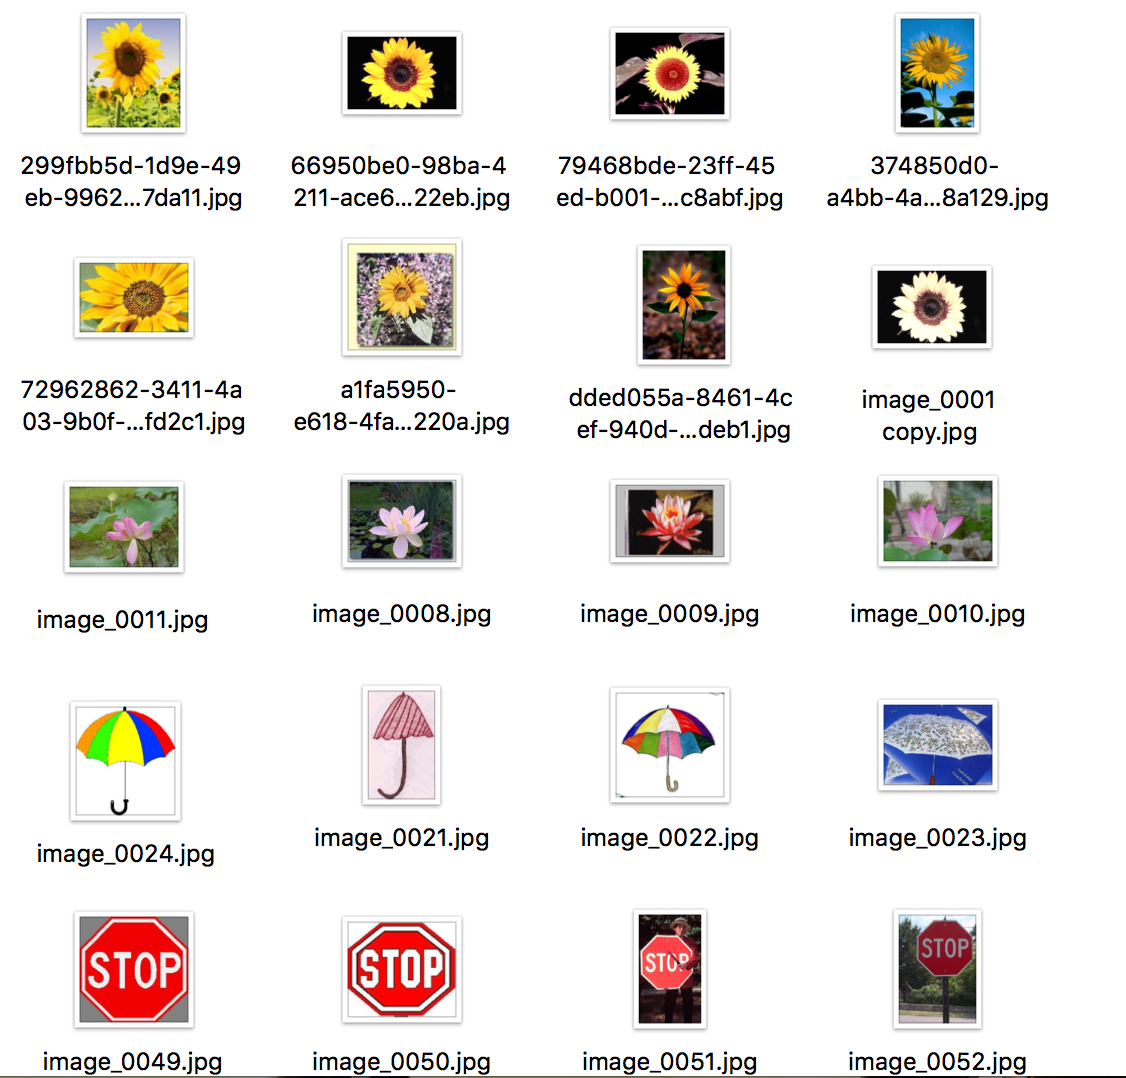
\includegraphics[scale=0.4]{figures/figure_1}
	\caption{Image dataset for the experiment}
\end{figure}

The query image is chosen to be the sunflower displayed in the left top corner of Figure 2. Three modified version of this image were also added in the dataset: shrunk, low-saturation and high-contrast. The modified versions of the query image are regarded as the ``similar" images in the image database. The other 20 sunflower images are also considered as similar images. The 4 water lily images are the ``not-so-similar" images. Umbrella images and the stop-signs are the completely different images. If the umbrellas and stop-signs are picked as similar images, they will be treated as false-positives.

\begin{figure}[h!]
	\centering
	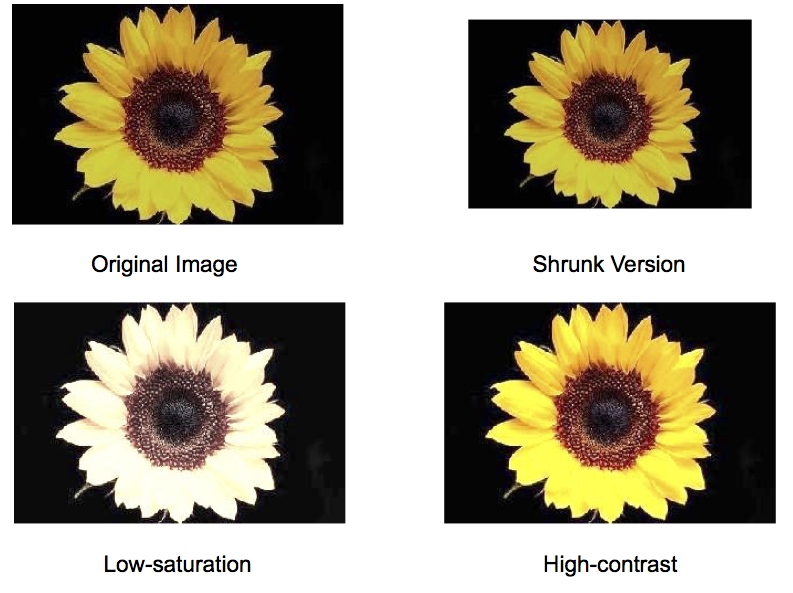
\includegraphics[scale=0.6]{figures/figure_2}
	\caption{Modified copies of the query image were added to the database as the similar images}
\end{figure}

The Image class from PIL is used to load the images off disk. Then the ImageHash python library  \url{https://github.com/JohannesBuchner/imagehash} will provide the aHash, pHash and dHash functions. The images stored in the dataset will be iterated, three different hash values were computed for each image, and these hash values were stored in three shelve key-value databases: aHash.db, pHash.db, dHash.db. Given a query image, the hash value of this query image will be looked up in the corresponding database to search for the similar existing hash values. The file name of the similar images could then be extracted from the Python dictionary.

After the hash value of the query image is computed, a key question here is to define the ``similarity" between two images using their hash values. The most straightforward measurement of similarity is the Hamming distance of the two hash values. The Hamming distance computes the number of bits that are different in two strings. Two images that have a smaller Hamming distance will be substantially more similar than images that have a large Hamming distance.

In the first trial, a Hamming distance of 5 is set as the threshold distance between two hash values to define two images are similar. The image search results within the image database are presented in Figure 3-5. Similarity search using the three hash algorithms all returns four results, which are the original copy of the query image and the three modified copies. It could be concluded that all of the three hash algorithms could generate promising image similarity search results.

\begin{figure}[h!]
	\centering
	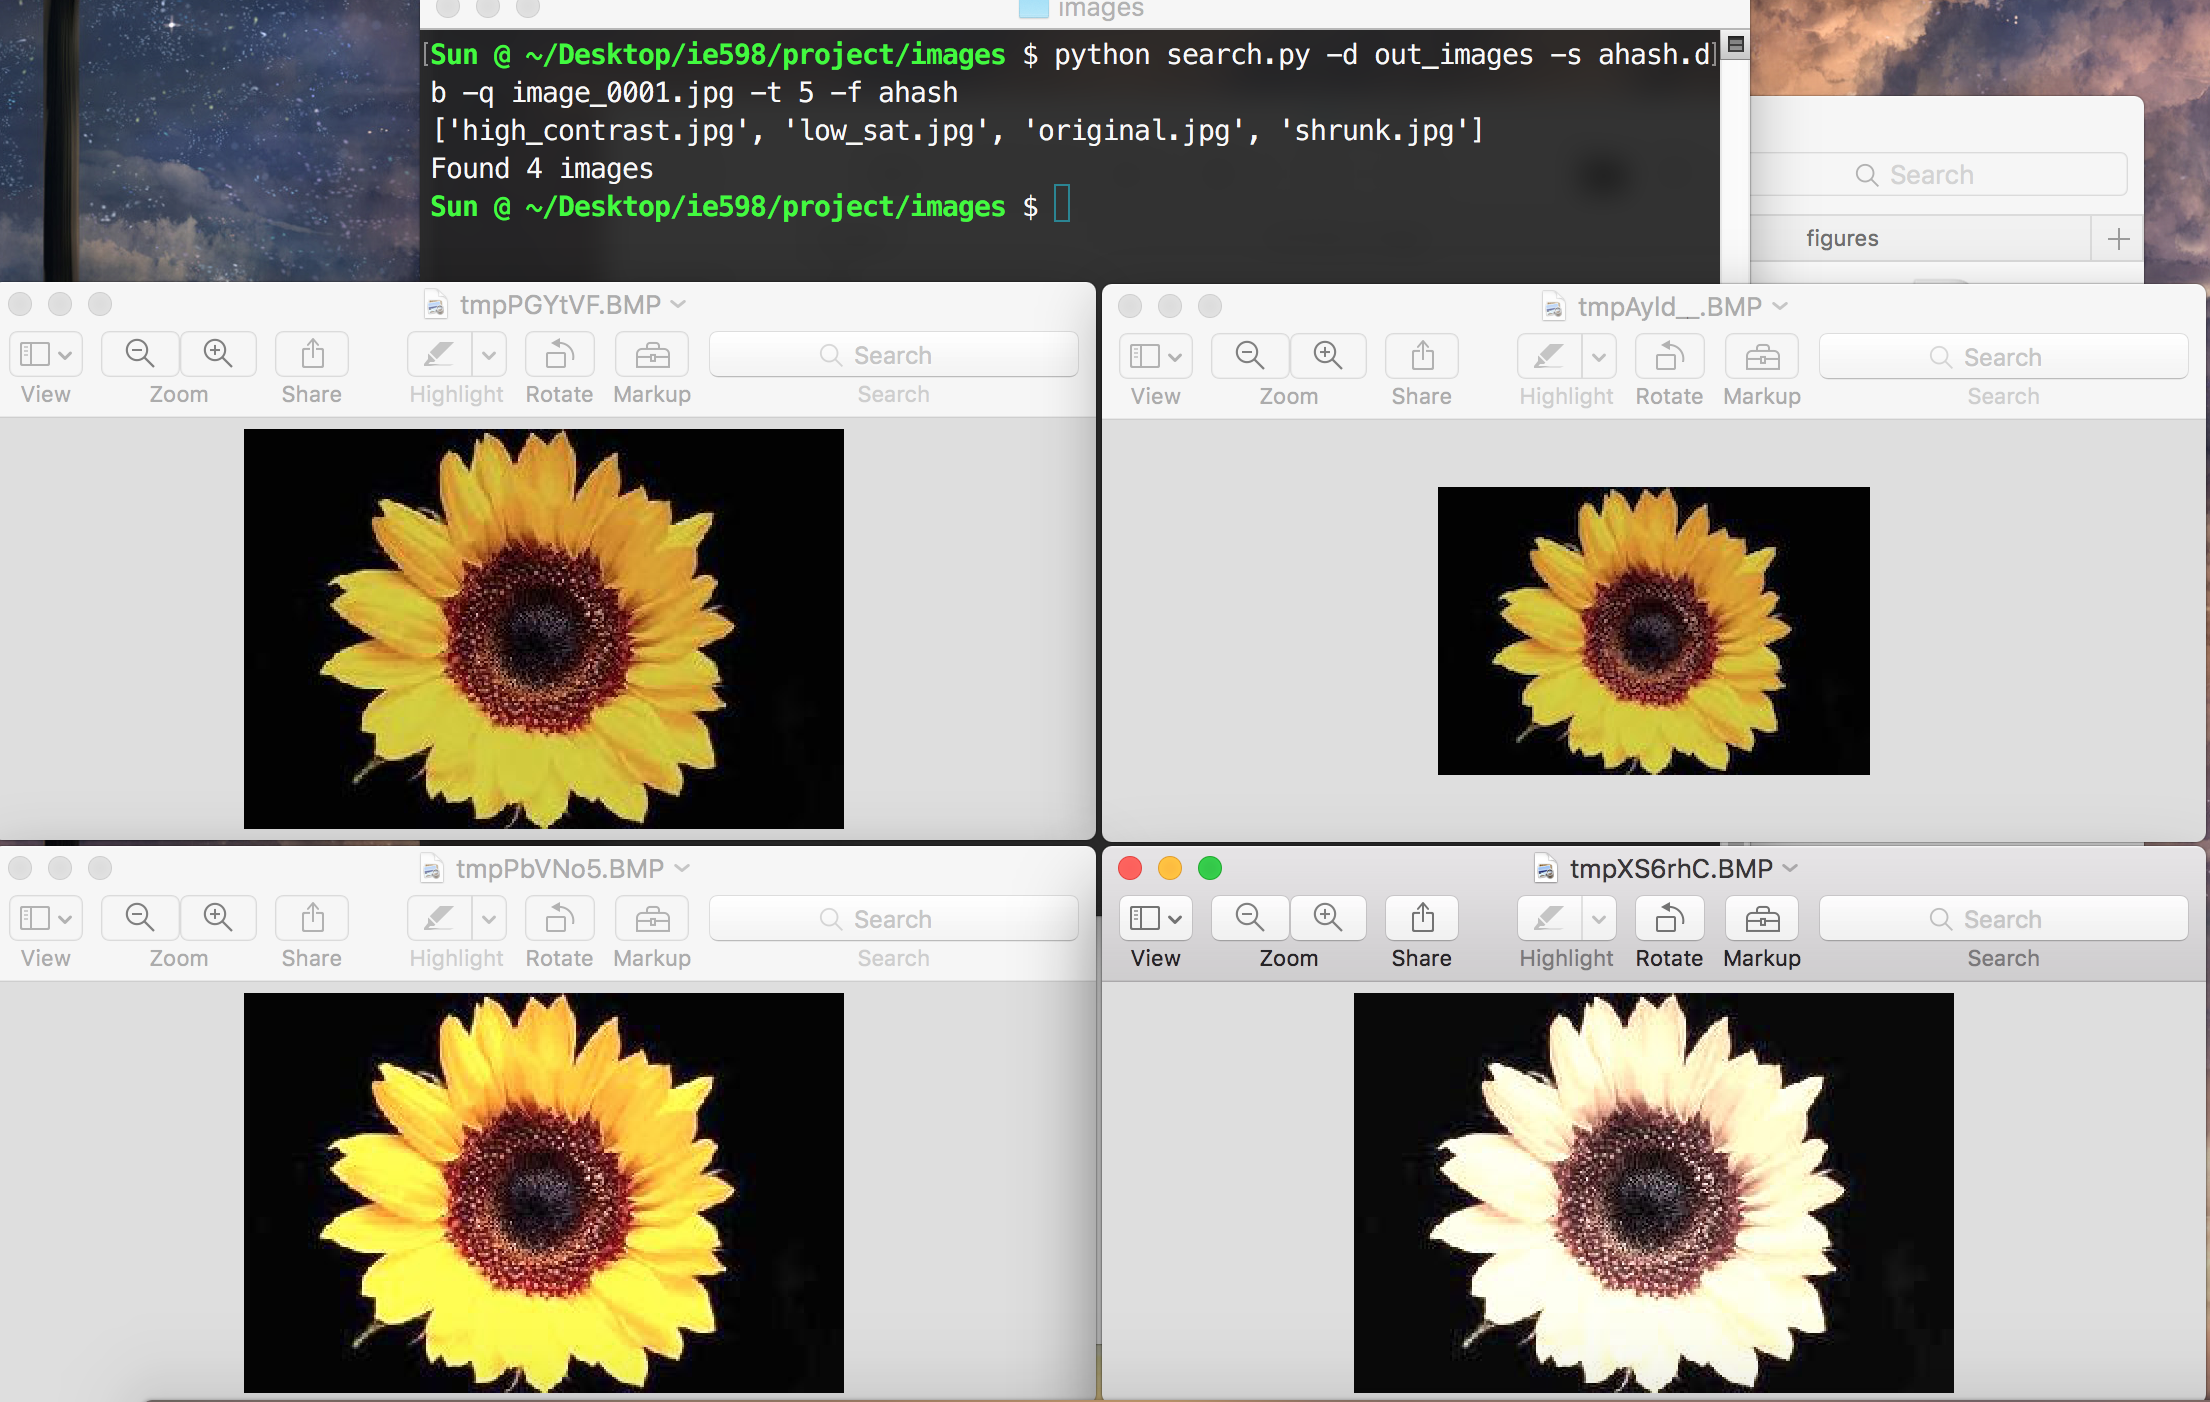
\includegraphics[scale=0.3]{figures/figure_3}
	\caption{Image similarity search results using aHash with Hamming distance less than 5}
\end{figure}

\begin{figure}[h!]
	\centering
	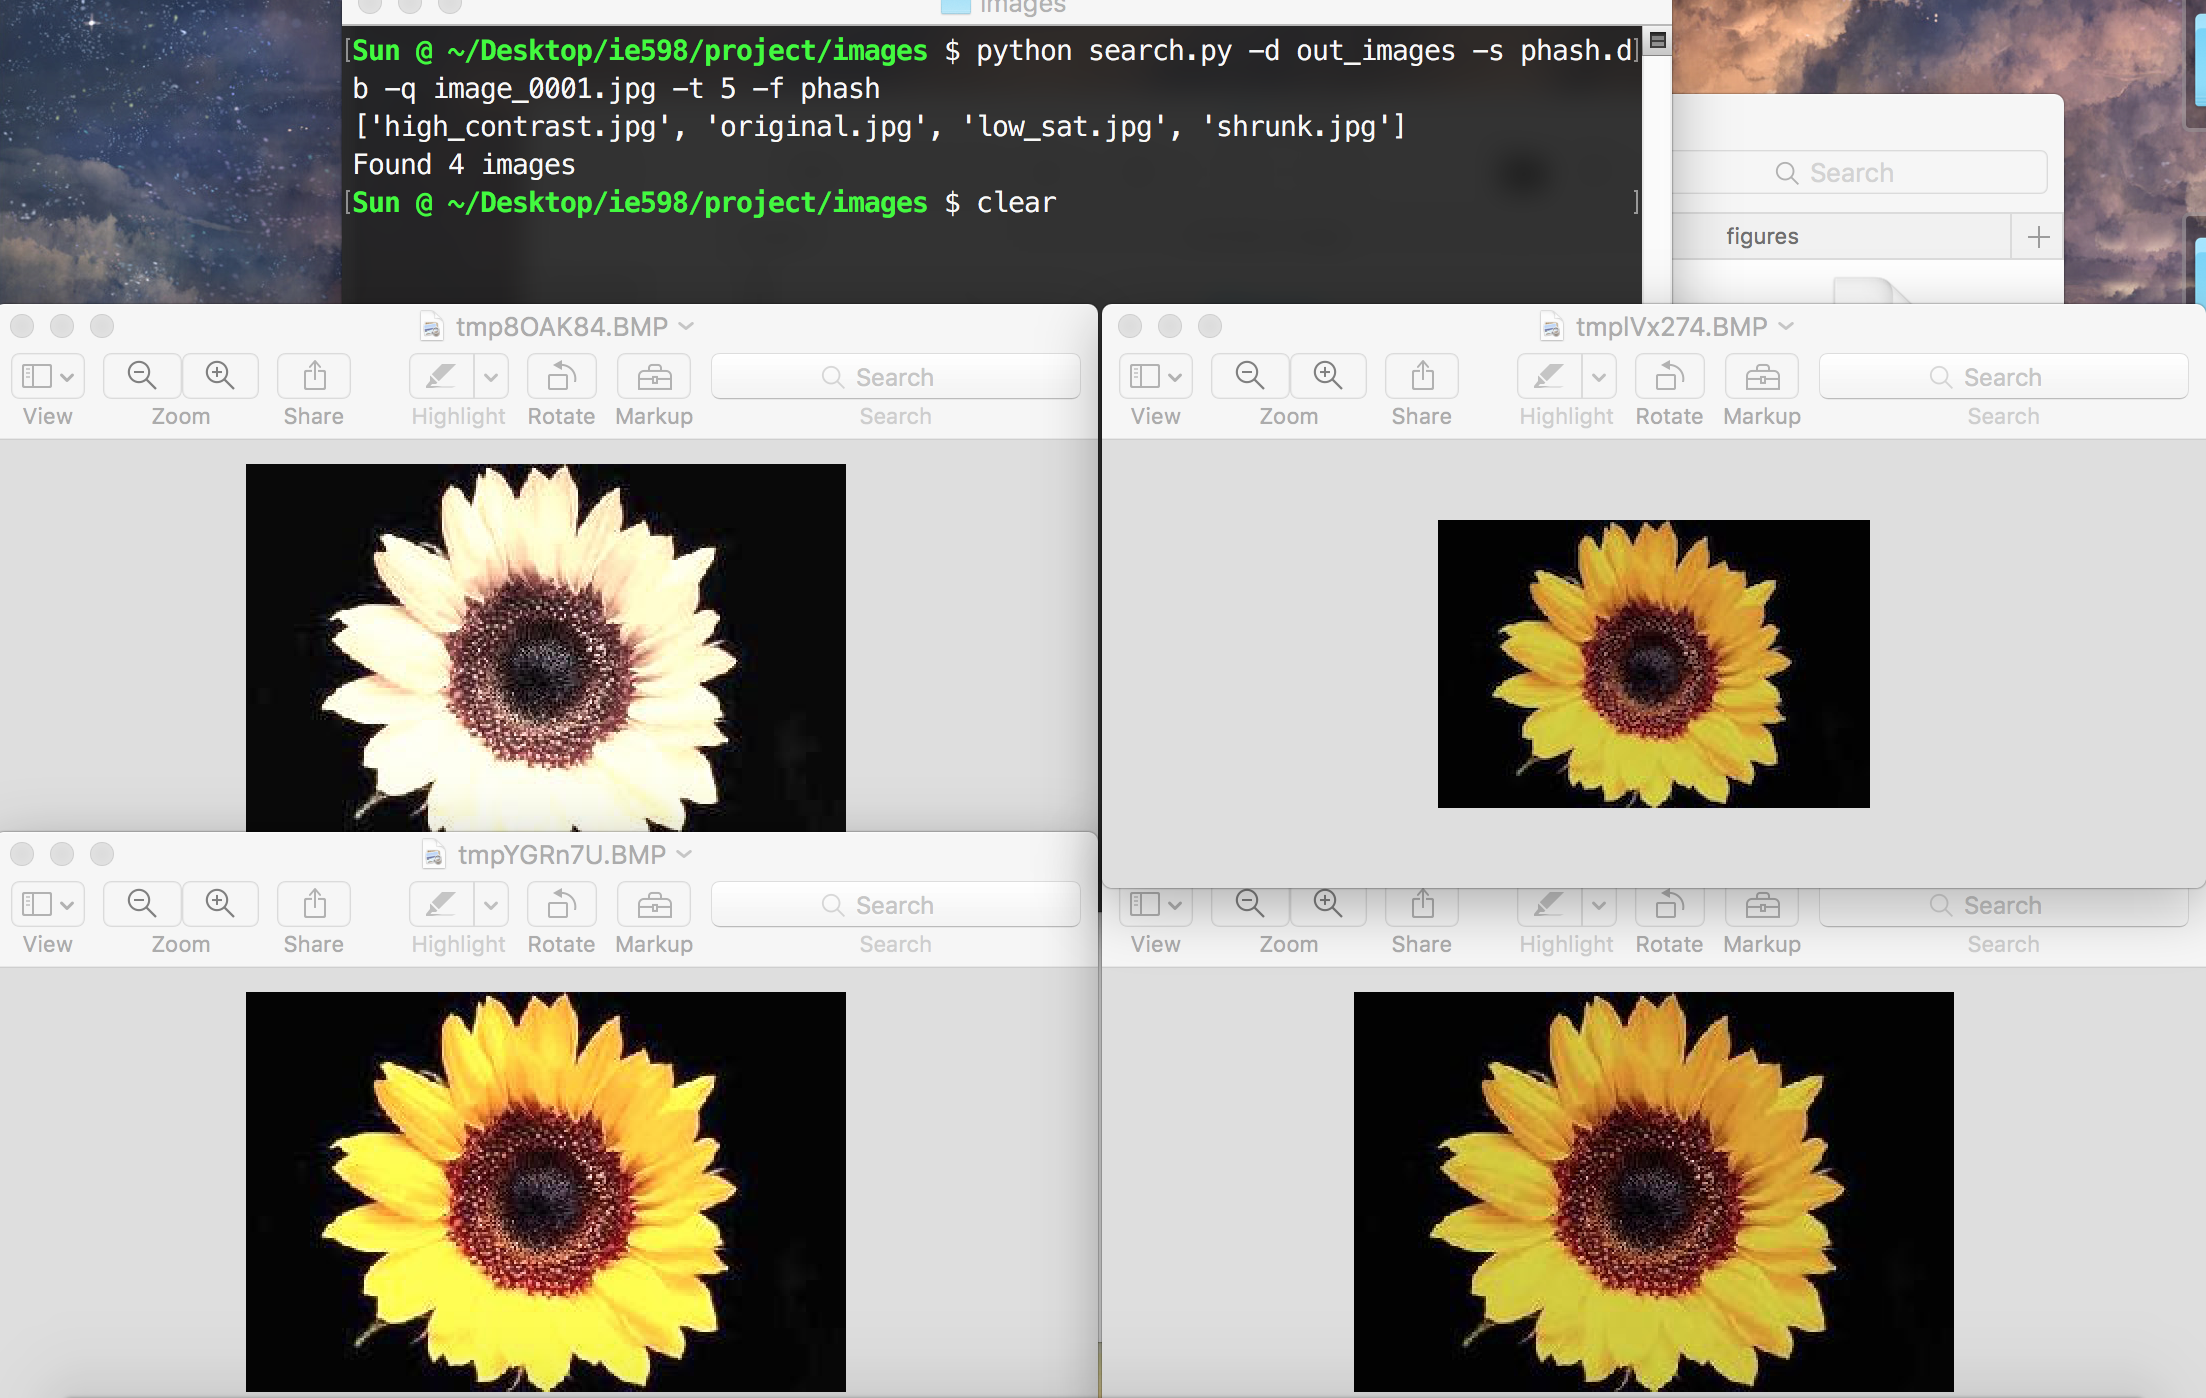
\includegraphics[scale=0.3]{figures/figure_4}
	\caption{Image similarity search results using pHash with Hamming distance less than 5}
\end{figure}

\begin{figure}[h!]
	\centering
	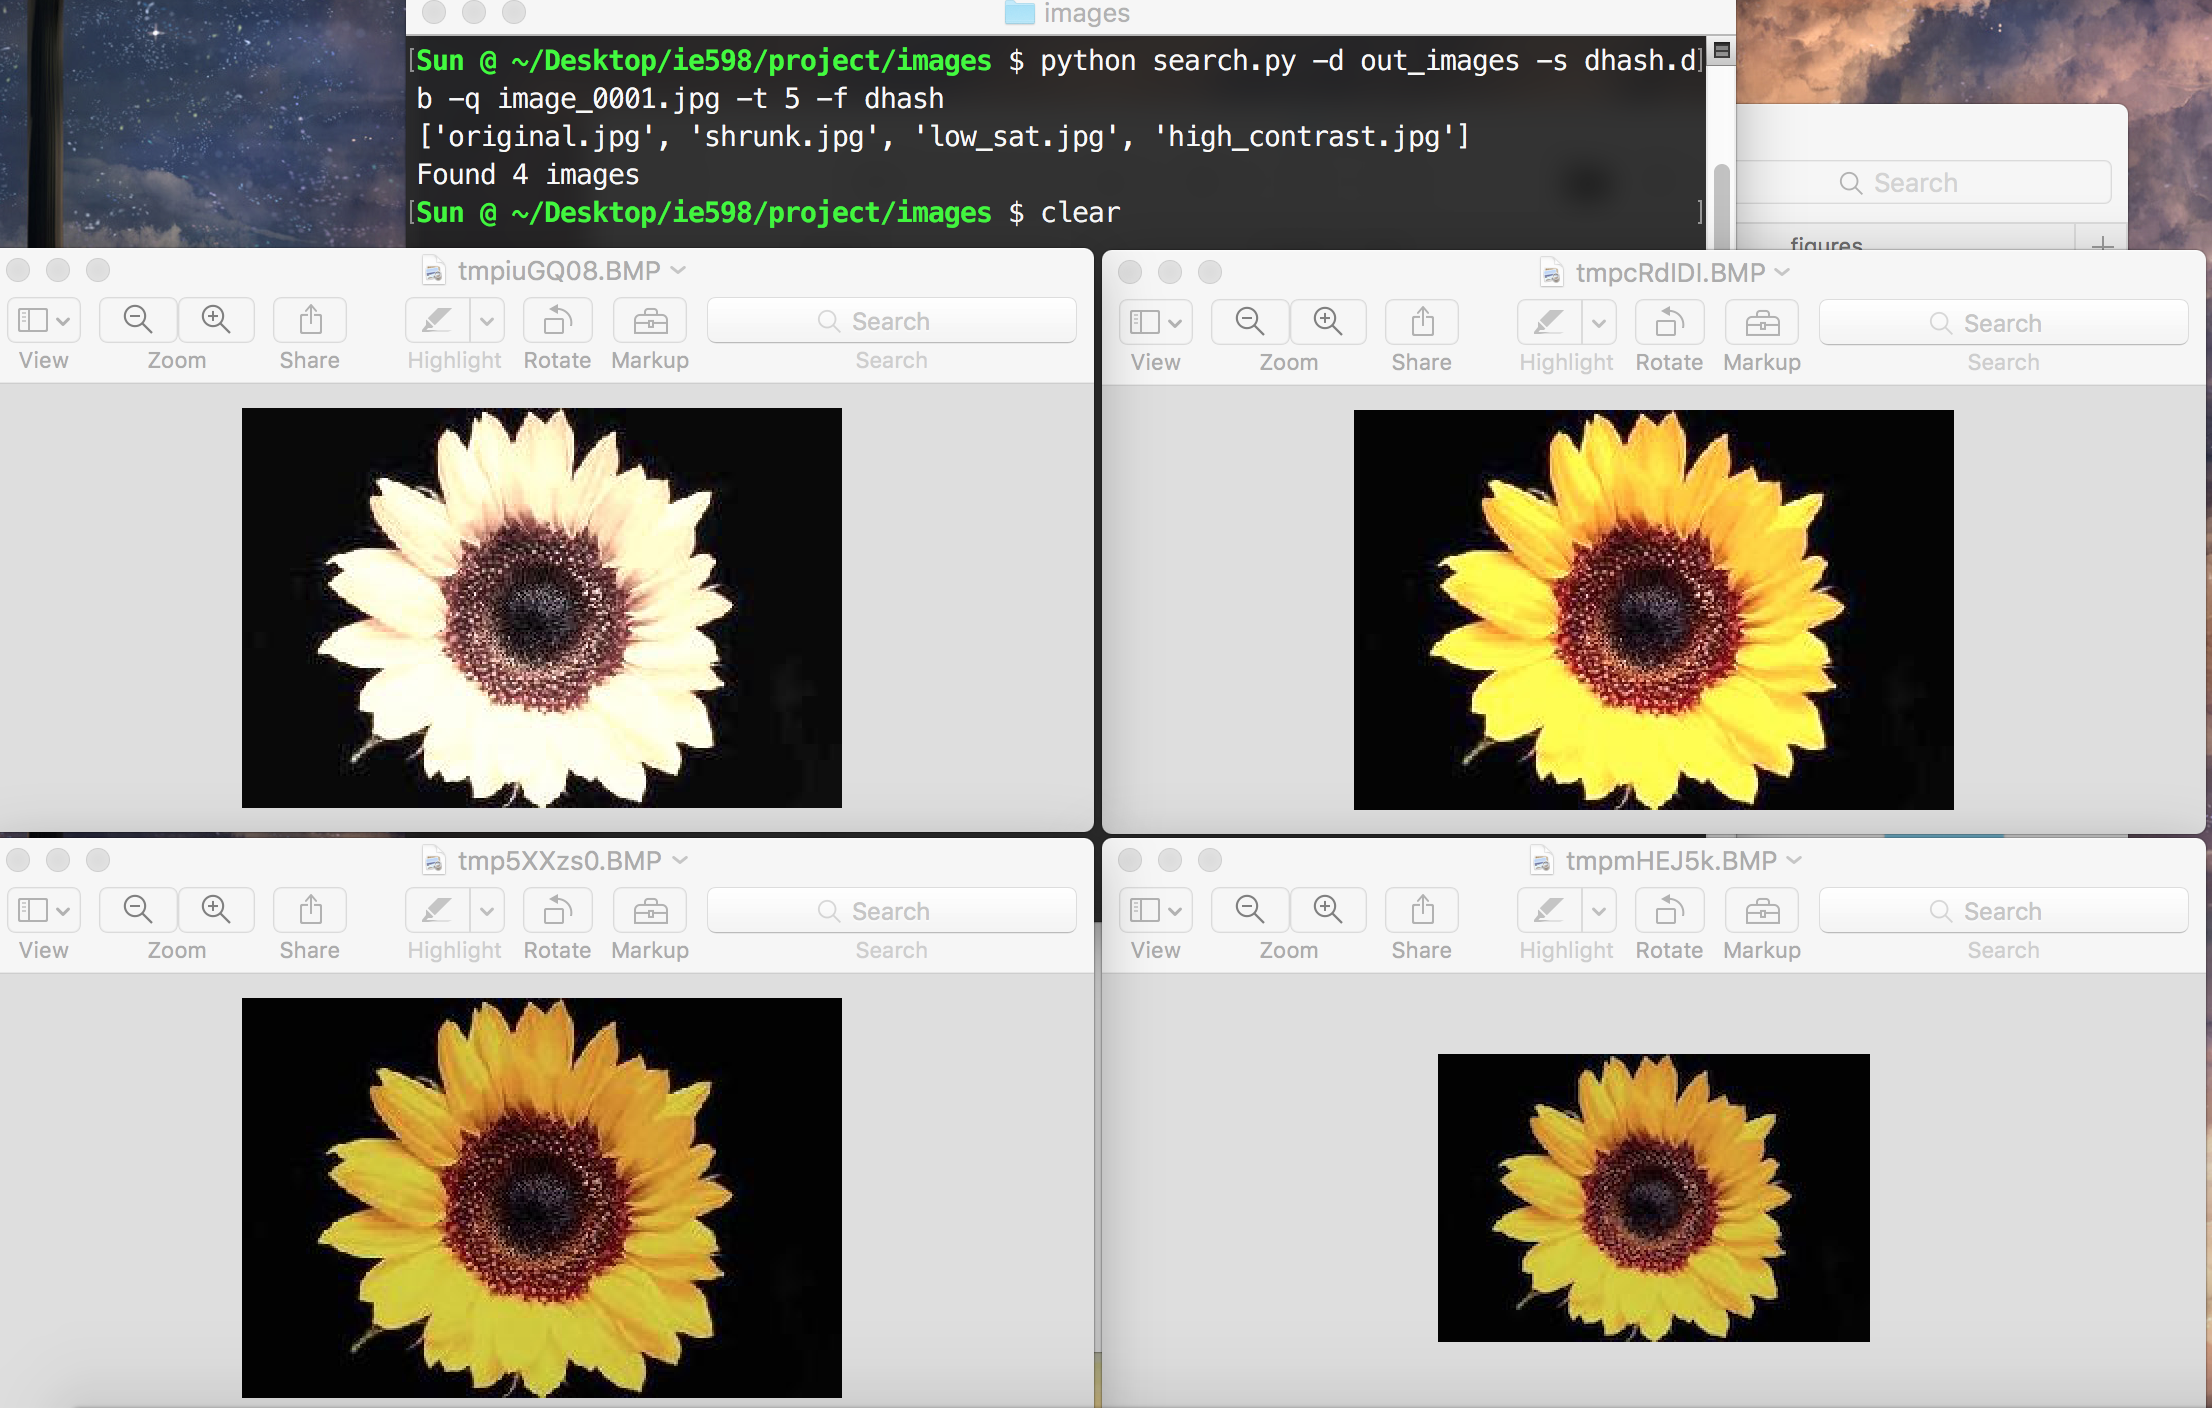
\includegraphics[scale=0.3]{figures/figure_5}
	\caption{Image similarity search results using dHash with Hamming distance less than 5}
\end{figure}

When the Hamming distance threshold is relaxed from 5 to 10, the image similarity search returns more images other than the original and modified copies of the query image. For example, similarity search using dHash returns 6 images, while the additional two images are also sunflowers and visually very similar to the query image. The two additional sunflower images are shown in Figure 6.

\begin{figure}[h!]
	\centering
	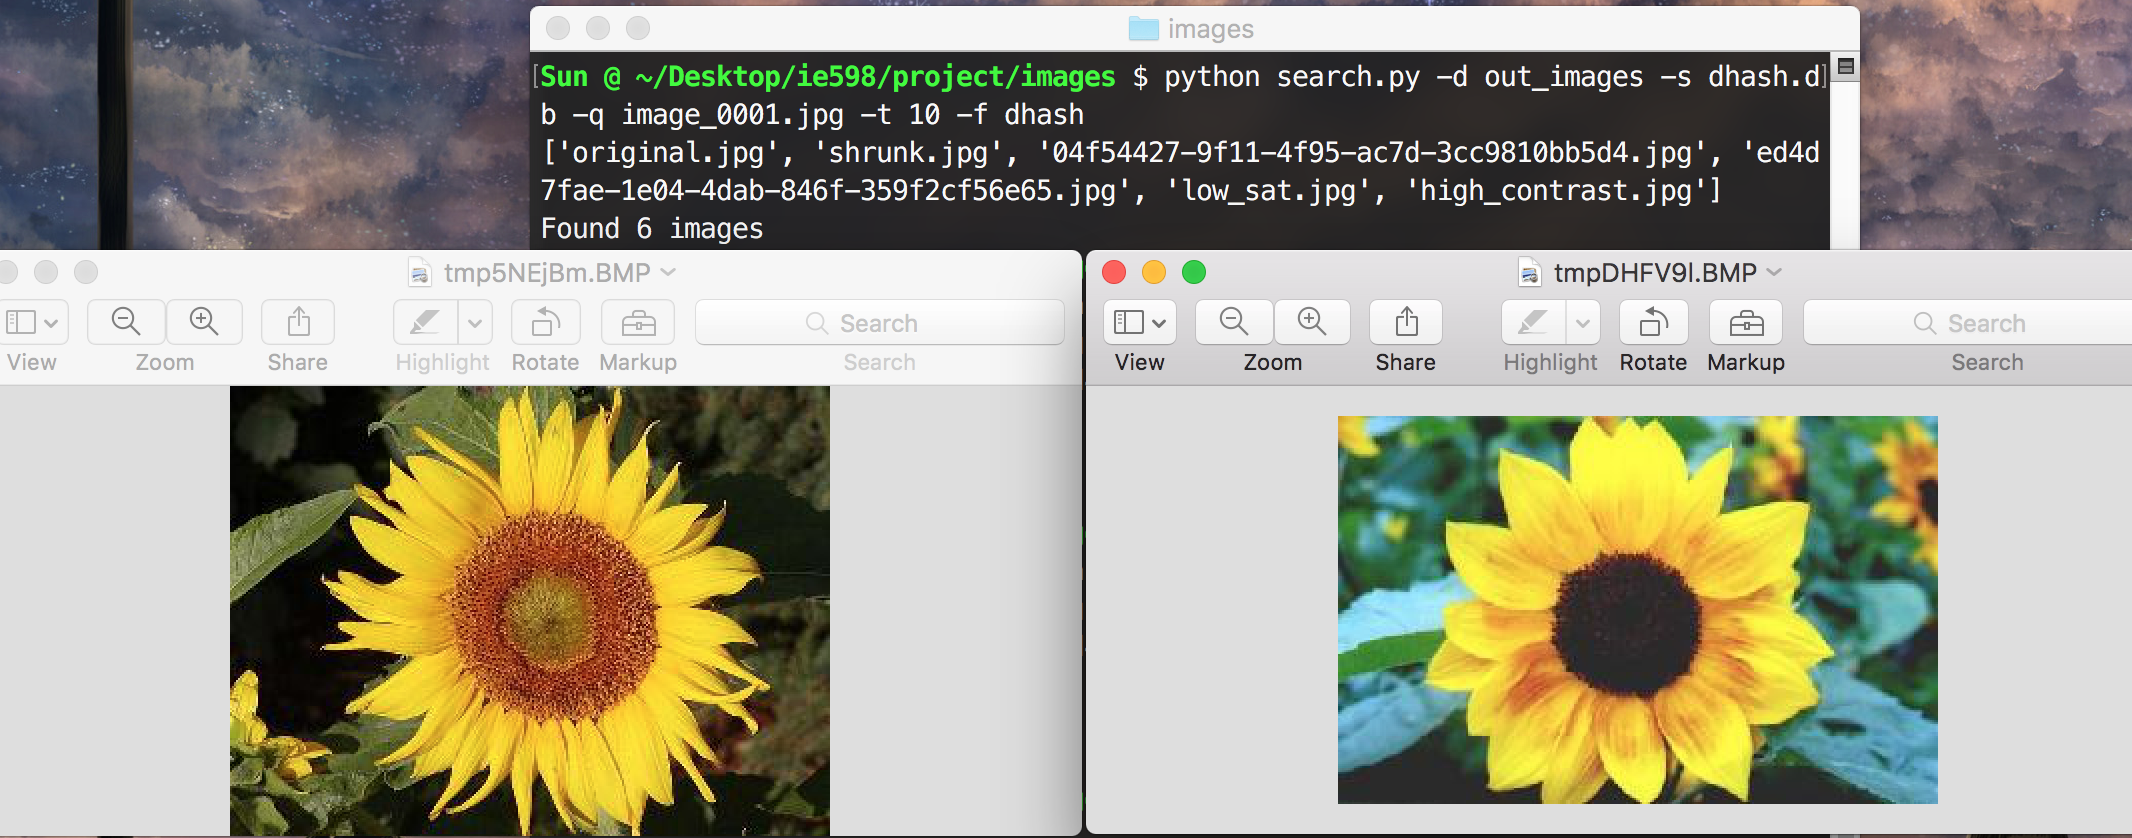
\includegraphics[scale=0.3]{figures/figure_6}
	\caption{Additional image similarity search results using dHash when the Hamming distance increases from 5 to 10}
\end{figure}

Therefore, the experiment results demonstrated that all of the three image hashing functions could successfully be used to conduct image similarity search in an image datasets. Lower threshold Hamming distance value would return images which are very similar to the query image, and higher threshold Hamming distance would return less similar images.

\section{MinHash Signature}

In this section, the approach of estimating the Jaccard Similarity between two sets using their MinHash signatures introduced in the course notes is extended to compare two sets of images.

The MinHash signature has a property that the probability of two sets having the same value of the MinHash signature is
equal to their set overlap, i.e., the ratio of the cardinalities
of the intersection and union of the two sets  \cite{chum2012fast}. In other words, the similarity of two image datasets could be approximately represented by the similarity of their MinHash signatures. Chum has proposed several computation methods of MinHash signatures for image datasets in 2012 \cite{chum2012fast}. In his implementation, the images are first represented as sets of visual words, and then different random permutations are performed over the vocabulary sets to generate the MinHash signatures. In order to achieve that, the image hashing methods introduced in the last section could be applied here. 

In my implementation, I combined the random hash functions proposed by \href{http://mccormickml.com/2015/06/12/minhash-tutorial-with-python-code/}{Chris McCormick} and the dHash image hashing algorithm to generate the MinHash signatures for the images.  

First, the images in the datasets were converted into hash values using dHash hashing algorithm. Each of the hash values represents an image. The hash value is then re-hashed into an 8-digit integer by implementing 

$\boldsymbol{imageID = abs(hash(imagehash)) \% (10 ** 8) }$

where the imageID represents a unique 8-digit integer for each image in the datasets.

These imageID values are then used as the seed for the hash functions used to generate the MinHash signatures. According to Chris, the hash function takes imageID as the input, and generates an output hash value:

$\boldsymbol{ h(imageID) = (a*imageID+b) \% c }$


The coefficients ‘a’ and ‘b’ are randomly chosen integers less than the maximum value of ImageID, and ‘c’ is a prime number slightly bigger than the maximum value of ImageID. For different choices of ‘a’ and ‘b’, this hash function will produce a different random mapping of the values. It is able to generate as many of these random hash functions as we want by choosing different values of ‘a’ and ‘b’.

10 random hash functions were used to compute the MinHash signatures. For each of the random hash functions, the minimum hash value produced among all of the images will be used as one component of the MinHash signature. When we are using 10 random hash functions, it will generate a MinHash signature with 10 components. 

The same 10 hash functions will be used on both of the two image datasets, and the signature for each dataset is computed and stored. In order to estimate the similarity between two image datasets, one should just count the number of signature components in which they match. The similarity of their MinHash signatures would provide a good estimate for their Jaccard Similarity.

In the experiment, I prepared two image datasets, each consists of 25 distinct images. These two datasets have 24 images which are the same, and each dataset has 1 unique image. Their actual Jaccard Similarity is 0.923, and this value will be estimated using their MinHash signatures.

\begin{figure}[h!]
	\centering
	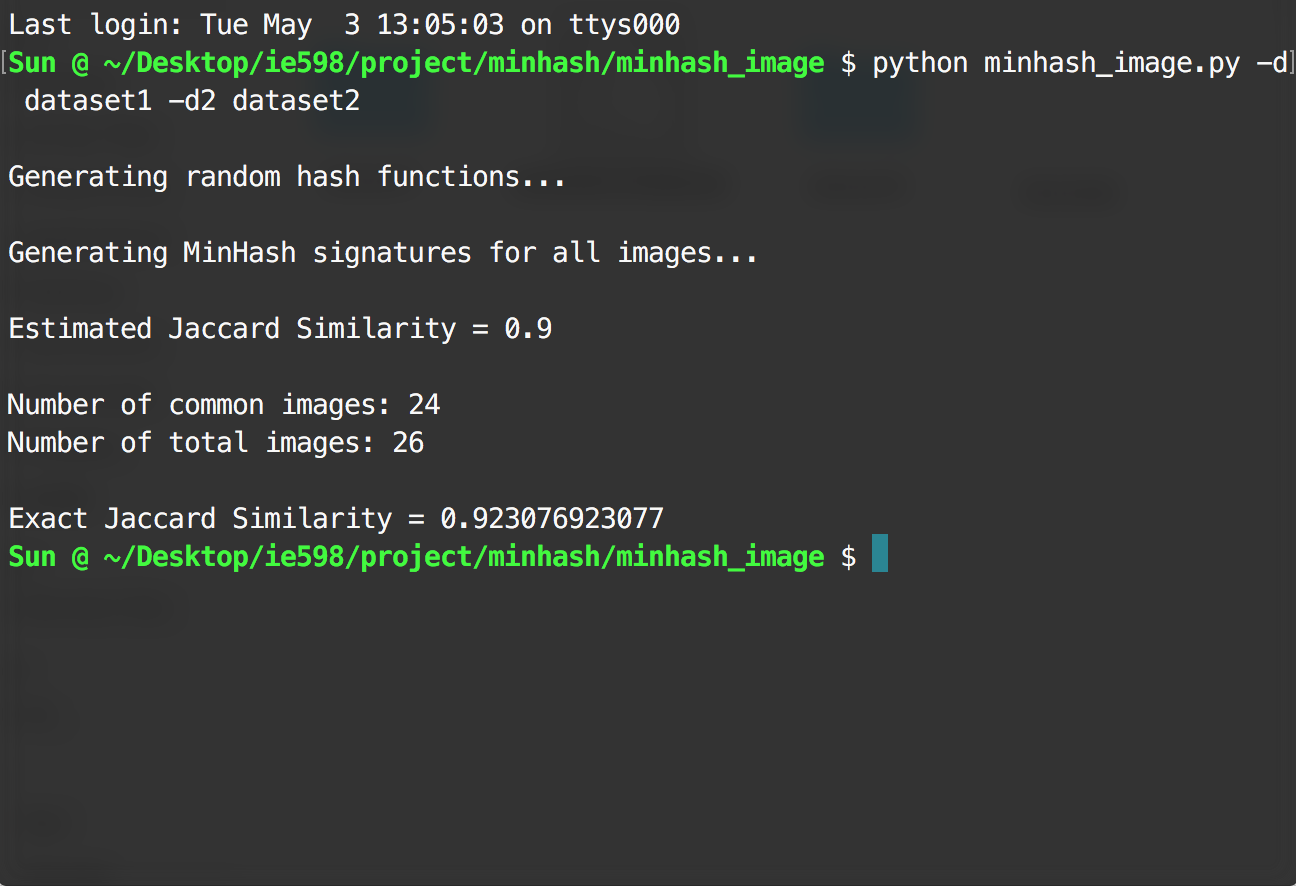
\includegraphics[scale=0.5]{figures/figure_7}
	\caption{Jaccard Similarity estimated using MinHash signatures}
\end{figure}

The estimation results are presented in Figure 7. It could be observed that the estimated Jaccard Similarity between two datasets is 0.9, which is pretty close to their authentic Jaccard Similarity. It should be noted that only 10 random hash functions were used to compute MinHash signature with 10 components, so the estimated similarity values are multiples of 0.1. The number of hash functions could be increased to improve the estimation precision. It should also be noted that since this is an estimated similarity result, multiple runs of the program could generates different estimations for the Jaccard Similarity. 

\section{Conclusions}
In this project, the concept of similarity search taught in class was applied to the measurement of similarity among images. In the first part of the project, three different types of image hashing algorithms were introduced and discussed. Experiments were conducted to examine the performance of these three image hash methods. During the experiment, three image databases were established by hashing the images in a dataset using different types of hashing methods. A query image is then used as the input to search through the databases. All of the three hashing methods were shown to be capable to successfully detect similar images to the input query image. The Hamming distance criteria could be adjusted to search for different levels of similar images.

In the second part of the project, the concept of MinHash signature was applied to measure the similarity between two image datasets. Images in the datasets were first hashed into sets of hash values, and the MinHash signature of each image dataset was computed by different random hash functions. By comparing the MinHash signatures of the image datasets, the Jaccard Similarity between two sets of images could be estimated. 

\bibliographystyle{unsrt}
\bibliography{ref.bib}


\end{document}


